\documentclass[journal, letterpaper]{IEEEtran}
%\documentclass{scrartcl}

\usepackage[ngerman,english]{babel}
%\usepackage[latin1]{inputenc}
\usepackage[utf8]{inputenc}
\usepackage[T1]{fontenc}
\usepackage{amsmath}
\usepackage{amsthm}
\usepackage{amsfonts}
\usepackage{tikz}
\usepackage{verbatim}
\usepackage{subcaption}
\usepackage{algorithm}
\usepackage{algorithmic}
\usepackage[pdftex]{hyperref}

\renewcommand{\algorithmicrequire}{\textbf{Input:}}
\renewcommand{\algorithmiccomment}[1]{\ \ // #1} % C-like // Comments

\hyphenation{render}

% No clubs and widows allowed
\clubpenalty10000
\widowpenalty10000
\displaywidowpenalty=10000

\begin{document}

%\title{Simulating elastic spheres without external forces}
%\subtitle{Project 1 for class CS6491 Computer Graphics}
\title{Swirl \\
	{\large Project 2 for class CS6491 Computer Graphics}}
%\author{Sebastian Weiss}
\author{Sebastian Weiss, Kristian Eberhardson\\ \today}
%\date{\today}

\maketitle

\begin{tikzpicture}[remember picture,overlay]
   \node[anchor=north east,inner sep=0pt] at (current page.north east)
              {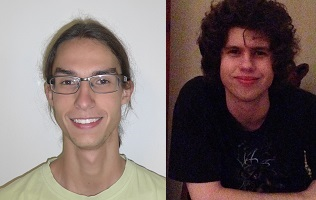
\includegraphics[scale=1.5]{pic}};
\end{tikzpicture}

\section{Objective}


\section{Input}

\section{Related interpolation schemes}

\subsection{Logarithmic spiral in 2D}

\subsection{Linear interpolation in 3D}

\subsection{Projected log spiral + Translation}

\section{Proposed model}

\subsection{3D rotation, first version}

\subsection{3D rotation, second version}

\subsection{Calculating $N$, $\alpha$ and $m$}

\subsection{Calculating $F$}

\subsection{Proof of steadiness}

\subsection{Dealing with special cases}

\subsubsection{No rotation}

\subsubsection{No rotation, no scaling}

\subsubsection{pure scaling}

\section{Results}

\end{document}